\documentclass[a4paper,11pt]{article}
\usepackage[utf8]{inputenc}
\usepackage[MeX]{polski}
\usepackage{hyperref}
\usepackage{graphicx}
\usepackage{pdfpages}
\usepackage{tikz}

\author{Michał Aniserowicz \href{mailto:michalaniserowicz@gmail.com}{{\small \nolinkurl{<michalaniserowicz@gmail.com>}}} \\ Jakub Turek \href{mailto:jkbturek@gmail.com}{{\small \nolinkurl{jkbturek@gmail.com}}}}
\title{{\Large [WEDT.A] Dokumentacja końcowa projektu} \\ Klasyfikacja stron WWW na podstawie struktury}
\date{30 maja 2013r.}

\begin{document}

\maketitle

\section{Temat projektu}

Tematem projektu jest automatyczna klasyfikacja stron WWW na podstawie struktury. W~ramach uścieślenia tematu projektu, wybrane do rozpoznowania zostały następujące kategorie stron internetowych:

\begin{itemize}
 \item dzienniki internetowe (\emph{blogi}),
 \item strony społecznościowe oparte na obrazkach (\emph{kwejki}),
 \item serwisy informacyjne,
 \item sklepy internetowe.
\end{itemize}

Projekt został wykonany w technologii Python 2.7.4 i~był testowany na systemach operacyjnych Windows~7 oraz Ubuntu~13.04. Projekt wykorzystuje bibliotekę PIL\footnote{Python Image Library - \href{http://www.pythonware.com/products/pil/}{http://www.pythonware.com/products/pil/}.} w~wersji 1.1.7.

\section{Implementacja}

\subsection{Schemat działania aplikacji}

Na następnej stronie przedstawiony został ogólny schemat działania programu. Obejmuje on dwie główne fazy działania aplikacji:

\begin{description}
    \item[uczenie się] Program generuje zestawienie wartości cech dla poszczególnych kategorii na podstawie próby wzorców.
    \item[klasyfikacja] Program dokonuje klasyfikacji pozostałych stron na podstawie wartości cech wyznaczonych w~poprzednim kroku.
\end{description}

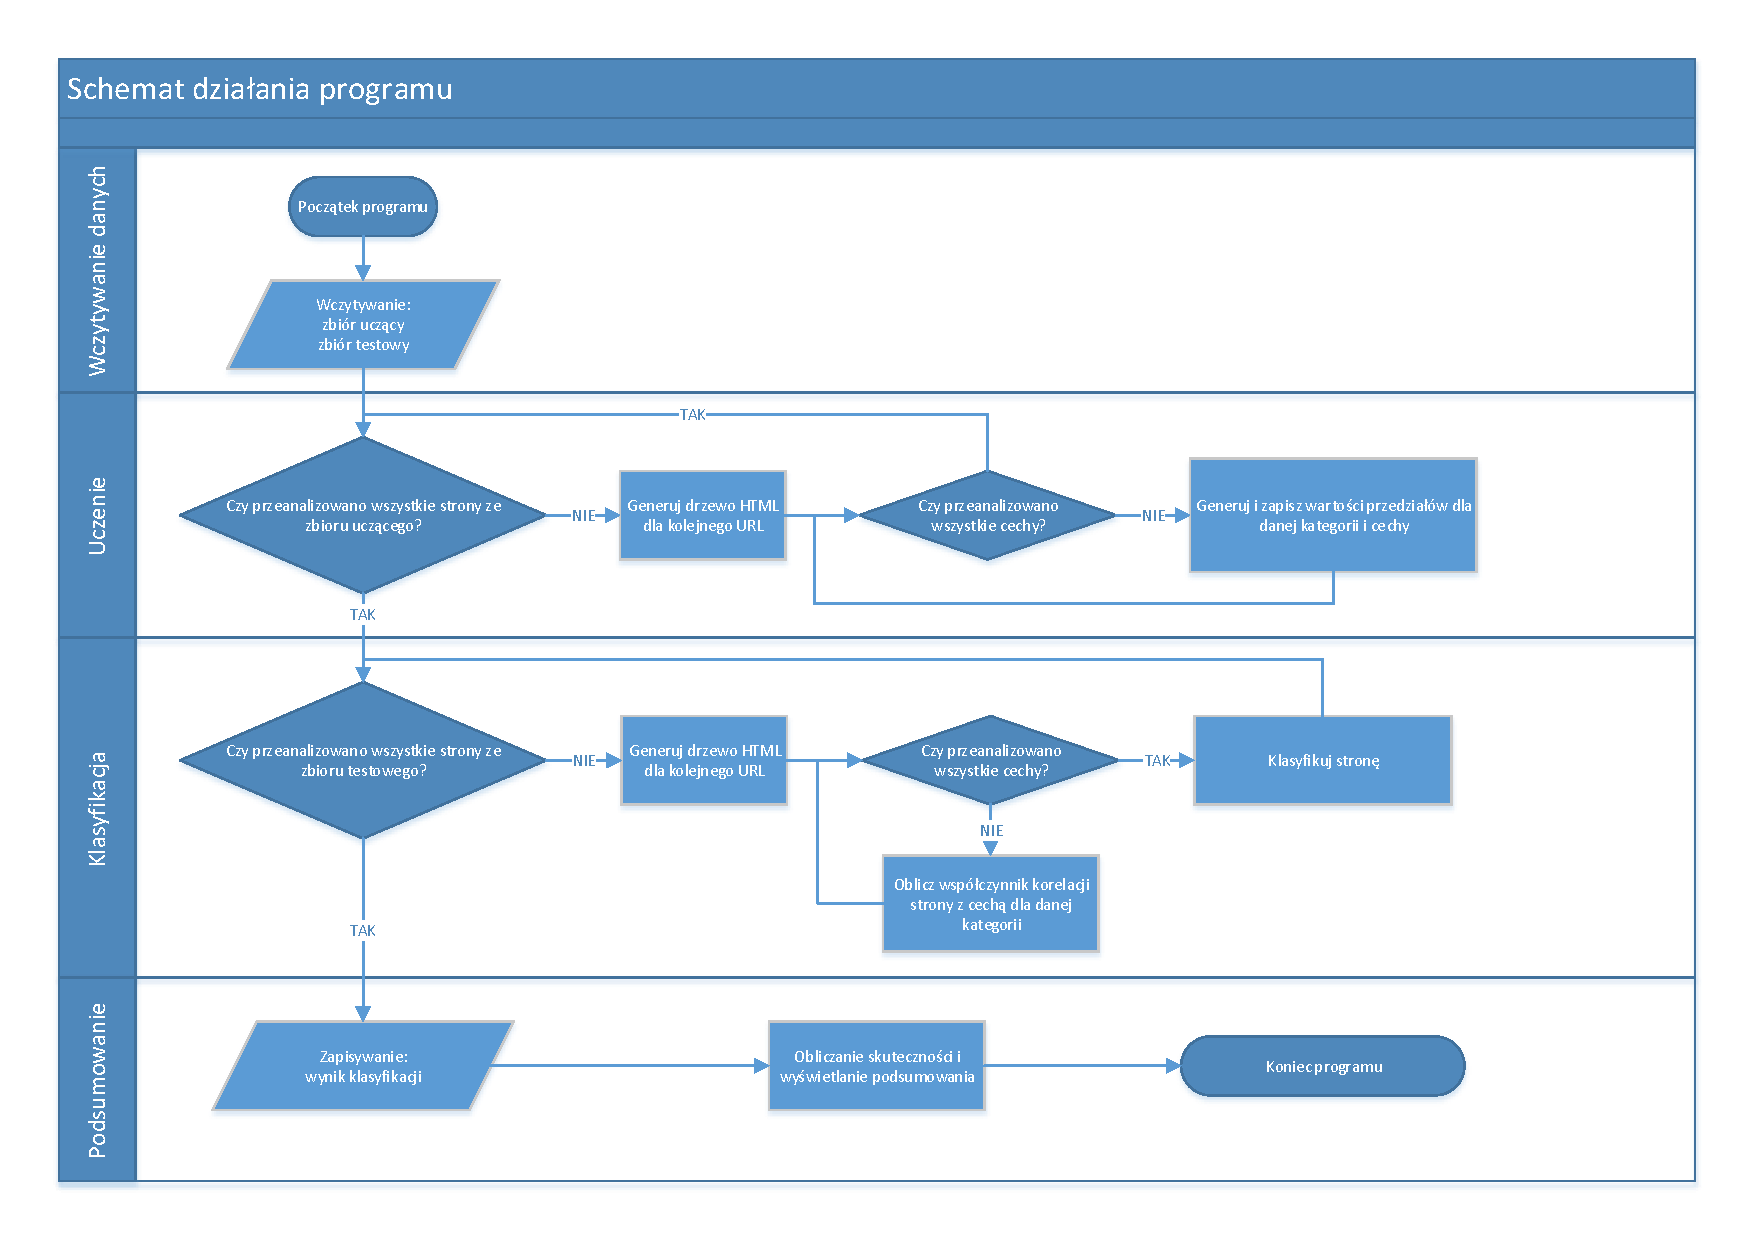
\includepdf[angle=90]{program_schema.pdf}

\subsection{Główna struktura strony}
\label{sec:main_structure}

Przed omówieniem zestawu cech badanych przez aplikację, należy wprowadzić pojęcie \emph{głównej struktury strony}, która będzie intensywnie analizowana. Główna struktura strony to najliczniejsza struktura, która posiada następujące cechy:

\begin{itemize}
    \item Występują w~niej wyłącznie tagi \verb+<td>+ lub \verb+<div>+, przy czym w~danej strukturze są to tagi wyłącznie jednego z~tych typów.
    \item Wszystkie tagi występują na jednym poziomie głębokości w~drzewie. Oznacza to, że mają wspólnego rodzica.
    \item Każdy z~tagów posiada jednakową wartość atrybutu \verb+class+.
    \item Każdy element struktury posiada więcej niż jeden element podrzędny lub większy niż jeden poziom zagłębienia elementów.
\end{itemize}

Główna struktura jest zaprezentowana na rysunku \ref{fig:structure}.

\begin{figure}[h!]
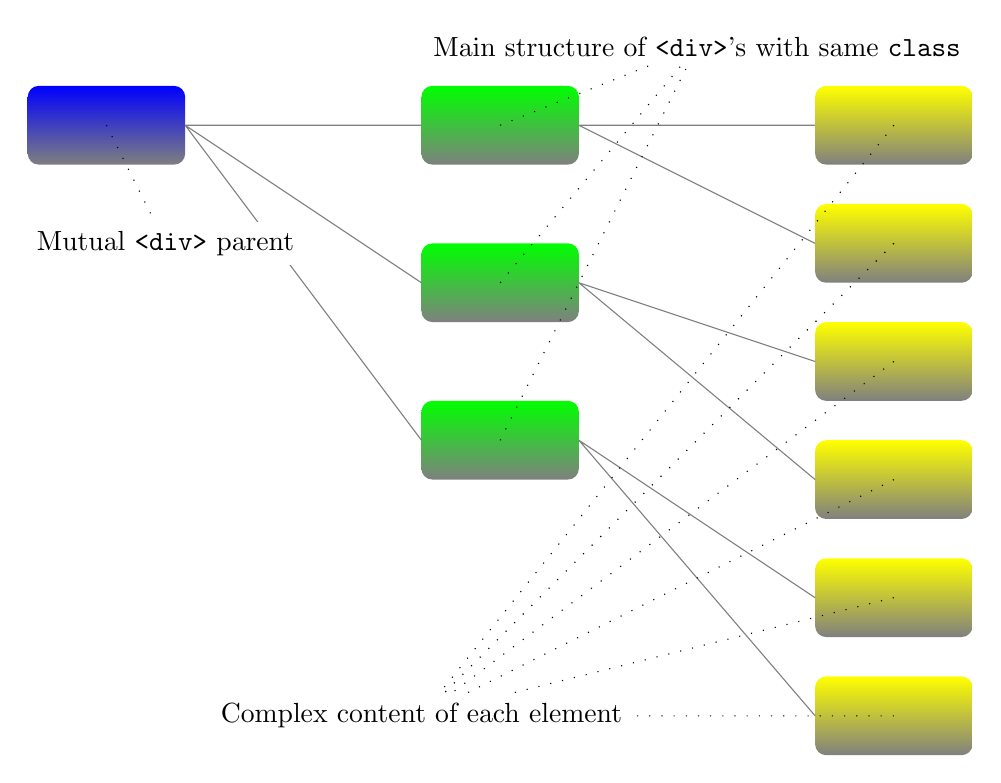
\begin{tikzpicture}
    \shade[rounded corners, top color=blue,bottom color=gray] (0,-1) rectangle (2,0);
    \shade[rounded corners, top color=green,bottom color=gray] (5,0) rectangle (7,-1);
    \shade[rounded corners, top color=green,bottom color=gray] (5,-2) rectangle (7,-3);    
    \shade[rounded corners, top color=green,bottom color=gray] (5,-4) rectangle (7,-5);       
    \shade[rounded corners, top color=yellow,bottom color=gray] (10,0) rectangle (12,-1);
    \shade[rounded corners, top color=yellow,bottom color=gray] (10,-1.5) rectangle (12,-2.5);    
    \shade[rounded corners, top color=yellow,bottom color=gray] (10,-3) rectangle (12,-4);    
    \shade[rounded corners, top color=yellow,bottom color=gray] (10,-4.5) rectangle (12,-5.5);    
    \shade[rounded corners, top color=yellow,bottom color=gray] (10,-6) rectangle (12,-7);    
    \shade[rounded corners, top color=yellow,bottom color=gray] (10,-7.5) rectangle (12,-8.5); 
    
    \draw[draw=gray]
        (2,-0.5) -- (5, -0.5)
        (2,-0.5) -- (5, -2.5)        
        (2,-0.5) -- (5, -4.5)
        (7,-0.5) -- (10, -0.5)
        (7,-0.5) -- (10, -2)
        (7,-2.5) -- (10, -3.5)
        (7,-2.5) -- (10, -5)
        (7,-4.5) -- (10, -6.5)
        (7,-4.5) -- (10, -8);
    \draw[loosely dotted] (1,-0.5) -- (1.75,-2) node[fill=white]
                        {Mutual \verb!<div>! parent};
    \draw[loosely dotted]
        (6, -0.5) -- (8.5,0.5)
        (6, -2.5) -- (8.5,0.5)
        (6, -4.5) -- (8.5,0.5) node[fill=white]
                        {Main structure of \verb!<div>!'s with same \verb!class!}; 
    \draw[loosely dotted]
        (11,-0.5) -- (5, -8)
        (11,-2) -- (5, -8)
        (11,-3.5) -- (5, -8)
        (11,-5) -- (5, -8)
        (11,-6.5) -- (5, -8)
        (11,-8) -- (5, -8) node[fill=white]
                        {Complex content of each element};
\end{tikzpicture}
    \caption{Zielone elementy należą do głównej struktury strony.}
    \label{fig:structure}
\end{figure}

Struktura ta jest charakterystyczna dla wszystkich czterech typów klasyfikowanych stron. Na \emph{blogach} zawiera treść wpisów, na \emph{kwejkach} obrazki, na stronach informacyjnych odnośniki do artykułów, natomiast w~sklepach internetowych - odnośniki do kategorii i/lub produktów.

\subsection{Analizowane cechy strony}

Na etapie uczenia się oraz klasyfikacji brane są pod uwagę, między innymi, następujące cechy:

\begin{itemize}
    \item Liczba elementów w~głównej strukturze strony.
    \item Liczba powtórzeń głównej struktury strony. Sprawdza czy struktura się powtarza i, jeżeli tak, to w~jakiej liczbie.
    \item Średnia ilość tekstu przypadająca na każdy element głównej struktury strony oraz jego dzieci. 
    \item Średnia ilość obrazów przypadająca na każdy element głównej struktury strony oraz jego dzieci.
    \item Liczba obrazów na stronie.
    \item Rozmiary największego oraz najmniejszego obrazu na stronie.
    \item Liczba odnośników na stronie.
    \item Stosunek długości tekstu zawartego w~odnośnikach do długości całego tekstu zawartego na stronie.
    \item Średnia długość lokalnego odnośnika\footnote{Odnośnik lokalny prowadzi do tej samej domeny, w~której znajduje się analizowana strona.} na stronie.
    \item Liczba tagów w~specyfikacji HTML5 (przykładowo: \verb+<article>+ oraz \verb+<section>+).
    \item Stosunek liczby odnośników do liczby obrazów na stronie.
    \item Stosunek długości tekstu do liczby obrazów na stronie.
\end{itemize}

Cechy te dobrze różnicują cztery zadane kategorie stron internetowych. Przykładowo serwisy informacyjne charakteryzują się wysokim współczynnikiem długości tekstu w~odnośnikach do całkowitej długości tekstów, długimi odnośnikami lokalnymi, dużą ilością obrazów na stronie oraz częstym występowaniem tagów w~specyfikacji HTML5. Dla kontrastu blogi charakteryzują się niewielkim stosunkiem liczby odnośników do długości tekstu, niewielką liczbą obrazków, dużą koncentracją tekstu w~głównej strukturze oraz większą niż dla serwisów informacyjnych liczbą elementów w~głównej strukturze strony.

\end{document}